\chapter{Contexte et analyse des risques}

\section{Introduction du chapitre}
Ce chapitre présente d'abord l'organisme d'accueil et le périmètre technique du projet, puis il formalise les risques liés aux accès privilégiés et l'objectif de sécurisation qui a guidé la conception.

\chapter{Representation CGI}

\section{Introduction du chapitre}
Ce chapitre introduit la representation CGI du projet (Contexte, Gouvernance, Implementation). Il sera complete avec le contenu detaille fourni ulterieurement.

\section{Objectif de la representation}
La representation CGI sert a presenter, en ouverture du document, une vue synthetique de la demarche:
\begin{itemize}
    \item \textbf{Contexte}: problemes de securite adresses et contraintes d'exploitation;
    \item \textbf{Gouvernance}: regles de decision, responsabilites et cycle d'approbation;
    \item \textbf{Implementation}: traduction technique dans l'architecture Zero Trust deployee.
\end{itemize}

\section{Elements a detailler (a completer)}
Le contenu final de cette section sera ajoute apres reception des elements attendus:
\begin{enumerate}
    \item definition operationnelle de la composante \textbf{C};
    \item definition operationnelle de la composante \textbf{G};
    \item definition operationnelle de la composante \textbf{I};
    \item articulation CGI avec les chapitres suivants du rapport.
\end{enumerate}

\section{Conclusion du chapitre}
La representation CGI pose le cadre de lecture du rapport et prepare l'analyse detaillee presentee dans les chapitres suivants.


\section{Perimetre critique}
Le périmètre critique concerne les serveurs d'administration, les machines cibles SSH, les composants réseau et les services de supervision utilisés pour les interventions de remédiation. Ces ressources concentrent les droits les plus sensibles et justifient un contrôle strict des élévations de privilège.

\section{Analyse des risques lies aux acces privilegies}
Trois scénarios principaux ont été retenus :
\begin{itemize}
  \item un compte permanent volé ou réutilisé abusivement ;
  \item une session privilégiée non tracée ou mal reliée à son initiateur ;
  \item une accumulation progressive de droits non révoqués.
\end{itemize}

\begin{figure}[H]
  \centering
  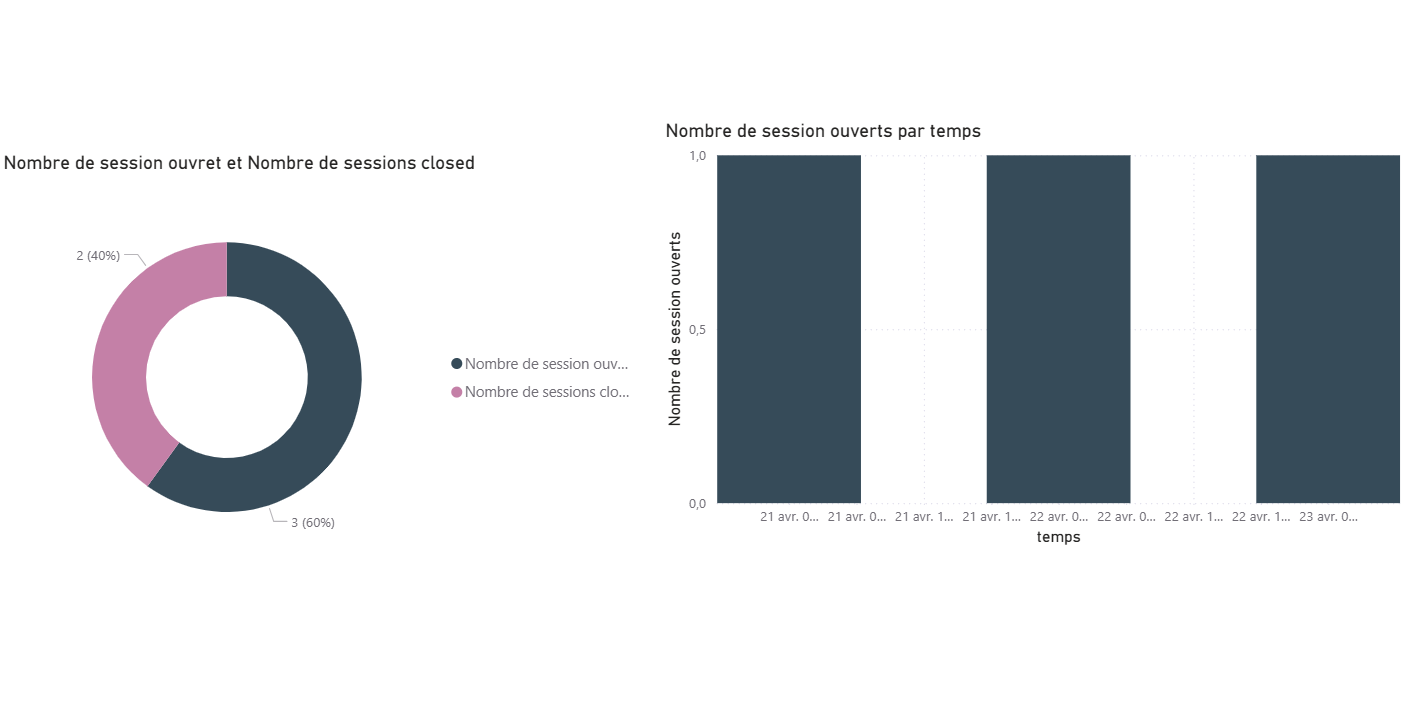
\includegraphics[width=0.95\textwidth]{images/Authentification IAM nombre de session ouvert et fermer dasn un anneau et dans des bar la bar est le nombre de session ouvert par temps.png}
  \caption{Synthèse Power BI des sessions IAM ouvertes et fermées dans le temps.}
  \label{fig:powerbi-sessions-iam}
\end{figure}

Cette vue met en évidence les volumes de sessions et leur évolution temporelle. Elle aide à justifier le passage vers une gouvernance Zero Trust avec limitation de durée et traçabilité explicite.

\section{Objectifs SMART du projet}
Les objectifs retenus sont les suivants :
\begin{itemize}
  \item supprimer les accès permanents non justifiés ;
  \item tracer 100\% des élévations de privilège ;
  \item imposer un TTL maximal configurable selon le type d'accès.
\end{itemize}

\section{Conclusion du chapitre}
L'analyse montre que la réduction de la surface d'attaque passe d'abord par la maîtrise des accès privilégiés, leur temporalité et leur journalisation. Ce constat motive directement le choix d'une architecture Zero Trust.